\documentclass[border=3pt]{standalone}
\usepackage{circuitikz}
\usetikzlibrary{calc}
\ctikzset{logic ports=ieee, logic ports/scale=0.9}
\begin{document}
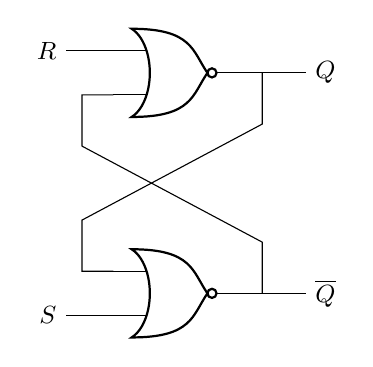
\begin{tikzpicture}[font=\sffamily\small]
  \node[nor port] (n1) at (0,1.4) {};
  \node[nor port] (n2) at (0,-1.4) {};
  % inputs
  \draw (n1.in 1) -- ++(-0.6,0) node[left]{$R$};
  \draw (n2.in 2) -- ++(-0.6,0) node[left]{$S$};
  % outputs
  \draw (n1.out) -- ++(0.9,0) node[right]{$Q$};
  \draw (n2.out) -- ++(0.9,0) node[right]{$\overline{Q}$};
  % cross-coupled feedback, crossing in the gap between the gates
  \coordinate (tq)  at ($(n1.out)+(0.35,0)$);
  \coordinate (tqb) at ($(n2.out)+(0.35,0)$);
  \coordinate (i1)  at ($(n1.in 2)+(-0.4,0)$);
  \coordinate (i2)  at ($(n2.in 1)+(-0.4,0)$);
  \draw (tq)  -- ($(tq)+(0,-0.65)$)  -- ($(i2)+(0,0.65)$)  -- (i2) -- (n2.in 1);
  \draw (tqb) -- ($(tqb)+(0,0.65)$) -- ($(i1)+(0,-0.65)$) -- (i1) -- (n1.in 2);
\end{tikzpicture}
\end{document}
